\documentclass{article}
\usepackage[utf8]{inputenc}
\usepackage{geometry}
\usepackage{amsthm}
\usepackage{amsmath}
\usepackage{amssymb}

\usepackage{hyperref}
\hypersetup{
    colorlinks=true,
    linkcolor=blue,
    filecolor=magenta,      
    urlcolor=blue,
}

\theoremstyle{definition}
\newtheorem{definition}{Definition}[section]
\theoremstyle{remark}
\newtheorem{remark}[definition]{Remark}
\theoremstyle{remark}
\newtheorem{example}[definition]{Example}
\theoremstyle{plain}
\newtheorem{theorem}[definition]{Theorem}

\newcommand{\R}{\mathbb{R}}
\newcommand{\Q}{\mathbb{Q}}
\newcommand{\Z}{\mathbb{Z}}
\newcommand{\N}{\mathbb{N}}

\theoremstyle{definition}
\newtheorem{tldr}[definition]{TLDR}

\usepackage{graphicx}
\graphicspath{ {images/} }

\title{IGL Automaton and Numeration Systems Reference}
\author{Eric Ma}
\date{February 2019}
\newcommand{\term}[1]{\emph{\textbf{#1}}}
%%Use \term to highlight new terminologies.
\begin{document}

\maketitle

\section{Glossary}
\subsection{Word and Property}
\begin{definition}
An \term{alphabet} is a set of \term{symbols}. Given an alphabet $\Sigma$, a \term{word} (or \term{string}) is a finite sequence of symbols in $\Sigma$. The \term{length} of a word $w$ is given by $|w|$, where $|w| \in \mathbb{N}$. For some symbol $a$, $|w|_a$ denotes the number of occurrences of $a$ in $w$.
\end{definition}

\begin{definition}
A \term{language} with alphabet $\Sigma$ is a set of words with alphabet $\Sigma$. 
\end{definition}
\begin{remark}
Given an alphabet $\Sigma$, the language $L$ consists of all words with length $n$ is $\Sigma^n$.
\end{remark}
\begin{definition}
Let $x=x_1x_2\dots $ be a word. A \term{factor} (or \term{substring}) is any continuous sequence contained in $x$, i.e. $x_ix_{i+1}\dots x_j$ is a factor of $x$ for all $1\le i\le j$. Denote $x[i\dots j] = x_ix_{i+1}\dots x_j$ and $x[i] = x_i$ for $1\le i\le j $.
\end{definition}

\begin{definition}
A word $w$ over some alphabet $\Sigma$ is \term{balanced} if for every $a \in \Sigma$, and pair of factors $u$ and $v$ with $|u| = |v|$, $\left||u|_a - |v|_a\right| \leq 1$; that is, the number of occurrences in $u$ and $v$ differs by at most one.
\end{definition}

\begin{definition}
$p$ is a \term{period} of a finite word $x = x_1\dots x_n$ if $p > 0$ and $x[i] = x[i+p-1]$ for all $1\le i \le n-p+1$. 
\end{definition}

\begin{definition}
A infinite word $w$ is \term{periodic} if there exists a period $m$ such that for all $i\ge 1$ $w[i] = w[i+m]$.
\end{definition}

\begin{definition}
A infinite word $w$ is \term{ultimately periodic} if there exists a positive integer $k$ and a period $m$ such that for all $i\ge k$ $w[i] = w[i+m]$.
\end{definition}

\begin{definition}
A word $w$ is recurrent if every factor of $w$ occurs infinitely many times. 
\end{definition}

\begin{definition}
A periodic word has constant gaps if for every letter $\alpha$ there is a $n\in\N$ such that any 2 consecutive instances of $\alpha$ are $n$-apart.
\end{definition}

\begin{definition}
$e$ is an \term{exponent} of a finite word $x$ if $\frac{n}{e}$ is a period of $x$ with length $n$. Alternatively, $e = \frac{|x|}{p}$, for a period $p$ of $x$.
\end{definition}

\begin{example}
All periods of ``alfalfa'' are 3, 6, and 7.
The corresponding exponent of ``alfalfa'' are $\frac{7}{3}$, $\frac{7}{6}$, and $1$.
\end{example}

\begin{remark}
For the same finite word, we usually call its smallest period \emph{the} period, and its largest exponent \emph{the} exponent.
\end{remark}

\begin{remark}
Notation: We write $x^a$ to represent $xx\dots x$ where $x$ is written $a$ times. Also applies when $a$ is fractional, just write the last $x$ ``half-way through".
\end{remark}

\begin{definition}
A critical exponent of an infinite word $w$ is the supremum of the set of exponents of all factors in $w$. i.e. 
$$\sup\left\{\frac{|u|}{p} \text{$u$ is a factor of $w$ with period $p$}\right\}$$
\end{definition}

\begin{definition}
An infinite word is an \term{automatic word} if there is an automaton with output such that running $i$ (in some numeration system) on the automaton will give the $i^{th}$ digit of the infinite word. 
\end{definition}

\begin{definition}
The \term{continued fraction} of a positive number $x$ is a sequence of numbers $a_0a_1a_2\dots$ such that \[
x=a_0+\cfrac{1}{a_1+\cfrac{1}{a_2+\cfrac{1}{ 1+\cdots}}}
\]
We write this as : $x = [a_0; a_1,a_2,\dots]$.

If the sequence is infinite and ultimately periodic with repeating part $a_i\dots a_j$, then we write this as $x = [a_0;a_1,a_2,\dots \overline{a_i,\dots,a_j}]$.
\end{definition}

\begin{definition}
An irrational number is \term{quadratic} if it is the root of some quadratic equation with rational coefficient. (Though we should refer to those numbers as quadratic irrational numbers, for this project, we refer to them as quadratic numbers.)
\end{definition}

\begin{theorem}
The continued fraction of a irrational number is infinite. The continued fraction of a quadratic number is ultimately periodic. 
\end{theorem}

\begin{definition}
A \term{characteristic Sturmian word} with slope $\alpha$, $c_\alpha$, is defined recursively: 
\begin{figure}[h]
    \centering
    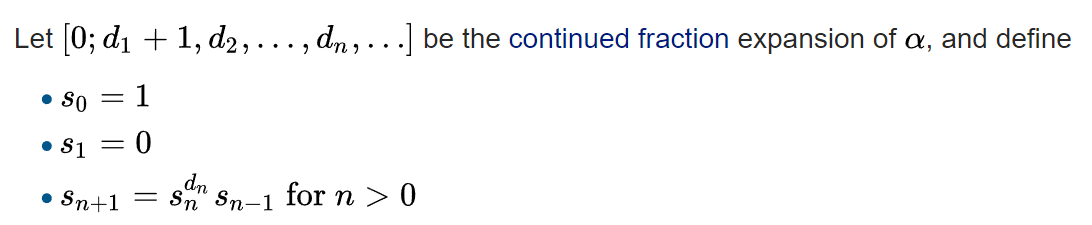
\includegraphics[width=0.7\textwidth]{characterSturmian.png}
    \caption{Characteristic Sturmian Word definition}
    \label{fig:characterSturmain}
\end{figure}

$c_\alpha$ is the limit of $s_n$ as $n\to \infty$.
\end{definition}

\newpage
\subsection{Automaton}
\begin{definition}
A \term{deterministic finite automaton}, or briefly a \term{DFA}, over alphabet $\Sigma$ is a quadruple $A = (S, I, T, F)$, where
	\begin{itemize}
		\item $S$ is a finite nonempty set called the set of \term{states}.
		\item $I$ is an element in $S$ called the \term{initial state}.
		\item $T \subseteq S \times \Sigma \times S$ is a nonempty set called the \term{transition table} or \term{transition diagram}.
		\item $F$ is a subset of $S$ called the set of \term{final states}.
	\end{itemize}
\end{definition}

\begin{definition}
A \term{non-deterministic finite automaton}, or briefly an \term{NFA}, over alphabet $\Sigma$ is a quadruple $A = (S, I, T, F)$, where
	\begin{itemize}
		\item $S$ is a finite nonempty set called the set of \term{states}.
		\item $I$ is a subset of $S$ called the set of \term{initial states}.
		\item $T \subseteq S \times \Sigma \times \mathcal{P}(S)$ is a nonempty set called the \term{transition table} or \term{transition diagram}.
		\item $F$ is a subset of $S$ called the set of \term{final states}.
	\end{itemize}
\end{definition}

\begin{tldr}
An automaton is something that looks like Figure \ref{fig:automaton1} or Figure \ref{fig:automaton2}. Circles are states. Arrows are transitions. Double circles are final states. An arrow with no source is pointing to the initial state.
\end{tldr}

\begin{figure}[h]
    \centering
    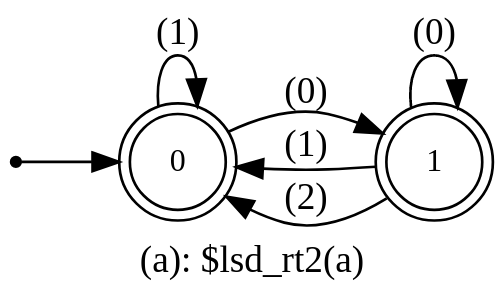
\includegraphics[width=0.25\textwidth]{lsd_rt2.png}
    \caption{Automaton 1}
    \label{fig:automaton1}
\end{figure}
\begin{figure}[h]
    \centering
    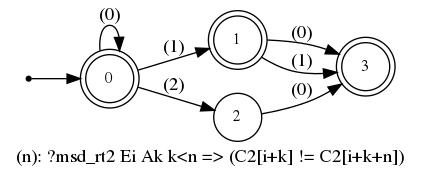
\includegraphics[width=0.5\textwidth]{theorem11_gv.jpg}
    \caption{Automaton 2}
    \label{fig:automaton2}
\end{figure}

\begin{remark}
Sometimes the alphabet is included in the definition of automata, but it doesn't matter as long as the alphabet is clear. 
\end{remark}
\newpage
\begin{definition}
Informal: A \term{run} of an automaton $A$ on a word $x$ is a sequence of states in the automaton, which starts at the initial state and follows the transition table until $x$ is used up. 
Formal definitions can be found in wiki page ``Automata theory". 
\end{definition}

\begin{definition}
A word $x$ is \term{accepted} by an automaton $A$ if the run of $A$ on $x$ stops on one of the final states.
\end{definition}

\begin{definition}
A language $L$ is \term{accepted} by an automaton $A$ if and only if every word in $L$ is accepted by $A$.
\end{definition}

\begin{definition}
An \term{automaton with output} is a deterministic finite automaton with outputs associated with all final states, and all non-final states transits to only non-final states. (Therefore, usually the non-final states are not drawn, and all states drawn are final states with output.) If a run of a word $x$ stops on a state with output $y$, we say that the output of the automaton with input $x$ is $y$. 
\end{definition}


\subsection{First-order Logic}

\subsection{Numeration Systems}
\begin{definition}
Let $\alpha$ be a quadratic number. Ostrowski Numeration System with slope $\alpha$ 
\end{definition}
\section{Walnut}
\textbf{Basic Usage}
\begin{itemize}
    \item  Change directory to the ``bin" folder under the Walnut folder. Run command ``java Main.prover" to start Walnut. 
    \item Use eval [name] ``[command]". To run command with name.
    \item Add $``?msd\_ns1"$ to use $ns1$ numeration system for numbers and variables.
    \item use $AW[i]$ to represent the $i^{th}$ number in the automatic word $AW$.
\end{itemize}

\section{Related theorems}
\subsection{Word property}
Feb. 11th Monday meeting:
\begin{theorem}
Critical exponent of $w$ is greater than or equal to $n$ iff there is a factor of the form $u^n$
\end{theorem}

\begin{theorem}
Any binary word with $\ge 4$ letters contains a square.
\end{theorem}

\begin{theorem}
There are infinite ternary square-free words. There are infinite binary cube-free words.
\end{theorem}

\begin{theorem}
For any exponent $\alpha > 1$, there is a word on a finite language that has critical exponent $\alpha$. (as $\alpha \to 1$, number of letters $\to \infty$.)
\end{theorem}

\begin{theorem}
For every infinite word $w_1$, there is a recurrent word $w_2$, such that every factor of $w_1$ is a factor of $w_2$.
\end{theorem}

\begin{theorem}
Every recurrent, aperiodic, balanced word on a finite language can be constructed as follows:

Let $u$ be an aperiodic Sturmian word on $\{a,b\}$. We replace the $a$'s by a periodic sequence with constant gaps, and likewise for the $b$'s.
(One letter replaced by one letter).
\end{theorem}
\section{Meeting Notes}
\subsection{Feb. 20th note:}
\begin{enumerate}
    \item Find ways to make the production of $x_k$ and/or $x_k$ automaton itself more efficient, so that we can actually use them. 
    \item What Walnut did with statement ``$C2[x]=C2[y]$" is basically ``$(C2[x]=@0 ~\&~ C2[y]=@0)~ | ~(C2[x]=@1 ~\&~ C2[y]=@1) \dots $". So no optimization here. 
    \item \begin{itemize}
        \item What we have:  \begin{enumerate}
            \item[(1)] Program that produces an addition-recognition automaton of Ostrowski Numeration System given a periodic continued fraction.
            \item[(2)] Program which produces $x_k$ for $k= 3,\dots, 10$.
            \item 
        \end{enumerate}
        \item What to do next: \begin{enumerate}
            \item[(1a)] Take 3-5 irrational quadratics and produce a paper with theorems analogous to the Fibonacci paper. Compare results across different quadratics, and make conjectures.
            \item[(1b)] Change the addition-recognition generator so that it produces a more general automaton that takes the quadratic number as arguments. (There is a sketch of proof that this can be done, but we want to know how complex will be).
            \item[(2a)] Try to get Walnut to produce and/or verify as many $x_k$'s as we can.
            \item[(2b)] Verify the experimental data and conjectures made about $x_k$'s critical exponents. 
            \item[(2c)] Can we determine a prefix of $x_k$ which is sufficient to verify $x_k$. 
            \item[(2d)] Reed and Eric: Send email to Philipp and Erik about obstacles with Task 2a,2b,2c. (cc everyone)
        \end{enumerate}
        \item Split Task: \begin{enumerate}
            \item[(1a)] Steve, Mihika, Dago
            \item[(1b)] Reed, Eric
        \end{enumerate}
        \item Need to meet Weekend. 
    \end{itemize}
\end{enumerate}
Some unimportant thought. 
Check first $n$ digits of $x_k$ and it's verified. 

\subsection{Feb. 24th note:}
Last semester, we tried replicating some of section 3 of the ``Fibonacci" paper using rt2-Ostrowski numeration system. The results are shown inside the ``Rt2 Word Theorem" folder on Box. Notice that not everything is correct. Thus what we want to do is:
\begin{enumerate}
    \item Fix the theorems proved in the box. 
    \item Replicate the rest of the paper using $\sqrt2$-Ostrowski.
    \item Replicate the paper using $\sqrt3$-Ostrowski (continued fraction $[\overline{1,2}]$). 
    \item Maybe replicate the paper using other numeration systems.
\end{enumerate}

To replicate the theorems, we want to follow the following steps:
\begin{enumerate}
    \item Read and understand the part in ``Fibonacci" paper that we want to replicate.
    \item Write predicates, and give explanations of what the predicate accepts.
    \item Run the predicates in Walnut.
    \item Explicitly interpret the result in Walnut, if feasible. 
\end{enumerate}
\href{https://app.box.com/folder/68301544796}{``Section 3.1 Theorems"} is a great example of what should be presented. \\

We want to try fixing the theorems in the box first, this includes writing and running the predicate, and giving explanation to the predicate and result. Here is a list of assignments of subsections in section 3 to everyone. Try to finish those (at least one subsection) before the Wednesday meeting. It should take about two hours to complete the task. 
 
\begin{itemize}
    \item Mihika: 10 3 
    \item Steve: 8 9
    \item Reed: 6 11
    \item Eric: 2 12
    \item Dago: 4 5
\end{itemize}

\subsubsection{Generating Addition and Verification Automaton for Ostrowski Numeration System}
\href{https://gitlab.engr.illinois.edu/2018IGL-automata/general-ostrowski-addition-automaton-java}{This program} can be used to generate addition and verification automaton for any Ostrowski numeration systems given the continued fraction of the quadratic irrational numbers. 
The general guide of how to use the program can be found in the readme file. Reach out to Eric if you want someone to show you how to use the program. 


\subsection{Feb. 27th note:}
\subsubsection{Midsemester Presentation Outline}
\begin{enumerate}
    \item Intro to numeration systems, with example preferring $\sqrt{2}$-Ostrowski. - Steve
    \item Definition of automaton and example of recognition automaton of $\sqrt{2}$-Ostrowski. - Mihika
    \item ``Intuitive" introduction to characteristic Sturmian word. give example of ``$C_{\sqrt{2}}$" - Reed
    \item A varied ``slice" of results from Walnut so far. - Dago
    \item Future work- i.e. the ``general addition automaton." - Eric
\end{enumerate}
To do: Try to write the slides for your part, if not good at Tex typeset, draw it and others can help. Keep your part in at most 2 slides. ++
\subsection{Mar 6th note:}
Things to improve:
\begin{enumerate}
    \item [Steve] Good. a little less
    \item [Mihika] Good. Go straight into examples.
    \item [Reed] Good analogy. 3 examples on the second slide instead of 5, went 1 minute over, maybe combine/speed up $2^{nd}$ and $3^{rd}$ slides.
    \item [Dago] Nice Slides, try to go quicker. 
    \item [Eric] Take a little less time, combine slides 1 and 2.
\end{enumerate}

\begin{enumerate}
    \item Think about Theorem 20 and 28
\end{enumerate}

\section{Mnemonic}
\begin{remark}
Sequence $1, 2, 5, 12, 29, \dots$: The $i^{th}$ number in this sequence is the value of the $i^{th}$ digit in $\sqrt{2}$-Ostrowski numeration system.
\end{remark}

\end{document}
